\chapter{Algorítmos Meta-Heurísticos e Inteligência de Enxames}

As técnicas de Inteligência de Enxames (IE) estão inseridas dentro Computação Evolutiva, apesar de trazer uma metáfora diferente da evolução das espécies. Na IE, o comportamento biológico de seres vivos serve de inspiração o que torna as técnicas de otimização mais simples e fáceis de serem implementadas do que as técnicas evolucionárias.

Chan e Tiwari (2007) \cite{chan2007preface}, em seu livro “Swarm Intelligence: Focus on Ant and Particle Swarm Optimization”, expõem que a complexidade crescente dos problemas exigiu que os pesquisadores encontrassem o possível formas de facilitar a solução dos problemas. Segundo os autores, isso motivou os pesquisadores a compreender ideias da natureza e implantá-lo nas ciências da engenharia. Esse modo de pensar levou a surgimento de muitos algoritmos biologicamente inspirados que provaram ser eficientes em lidar com os problemas computacionalmente complexos com competência, tais como Algoritmo Genético (GA), Otimização de Colônia de Formigas (ACO), Otimização de Enxame de Partículas (PSO), etc.

Na IA, de acordo com Eberhart e Kennedy (2001) \cite{eberhart2001swarm}, o comportamento global do enxame é um efeito emergente das interações locais dos membros do enxame. De acordo com Filho et al. \cite{bastos2008novel}, as informações pessoais e sociais guardam semelhança com operadores de recombinação e de cruzamento, enquanto que a conservação de movimento da partícula atua como uma espécie de mutação direcional. Há diferenças, no entanto, sendo a maior delas o papel da seleção natural: enquanto que métodos evolutivos tem como parte essencial a morte dos indivíduos menos aptos, em um processo social os indivíduos são preservados durante a execução do algoritmo, de forma que o próprio indivíduo se adapta no decorrer do tempo.

Há uma série algoritmos de otimização de problemas que abordam diferentes grupos de seres vivos, desde pássaros a vagalumes para resolver problemas de otimização. Engelbrecht (2006) \cite{engelbrecht2006fundamentals} exemplifica alguns problemas resolvidos pela IE como aproximação de funções, agrupamento, otimização de estruturas mecânicas, resolução de sistemas de equações, otimização de roteamento em redes de telecomunicações, coloração de grafos, programação e resolução do problema de atribuição quadrática, dentro outros. Os problemas aqui tratados são conhecidos tecnicamente por NP-difícil. Portanto, técnicas computacionais mais apuradas são necessárias para resolver esses problemas.


Dentro da IE, há várias técnicas que abordam diferentes grupos de seres vivos desde pássaros a bactérias. Entretanto, este trabalho faz uso das seguintes abordagens: \textit{ Ant Colony Optimization} (ACO), \textit{Particle Swarm Optimization} (PSO) e \textit{Fish School Search} (FSS). O ACO, Otimização por Colônia de Formigas, tem a sociedade organizada das formigas como modelo para busca de alimentos através de rastros deixados pelas formigas. Já o PSO, Otimização por Enxame de Partículas, tem como inspiração os bandos de pássaro, tendo como a forma de voar em grupo na busca de alimento e mecanismo de interação social. Por fim, o FSS \cite{bastos2009fish}, Busca em Cardume de Peixes, tem no movimento do nado dos peixes a inspiração para proteção e busca de locais mais favoráveis para sobrevivência.

% ---
\section{ACO}
\label{sec-aco}
% ---

O ACO, desenvolvido por Dorigo e sua equipe em 1996 \cite{dorigo1996any}, inspirou-se no comportamento de colônias de formigas reais, em particular, por seu comportamento de forrageamento. Uma das principais ideias é a comunicação indireta entre os indivíduos de uma colônia de agentes, chamados de formigas, com base em uma analogia com trilhas de uma substância química, chamada feromônio, que as formigas reais utilizam para a comunicação. As trilhas (artificiais) de feromônio são um tipo de informação numérica distribuída que é modificada pelas formigas para refletir sua experiência acumulada ao resolver um problema particular.

Como descreve Mulati, Constantino e da Silva (2013) \cite{mulati2013otimizaccao}, foi descoberto que a comunicação entre as formigas que caminhavam pela trilha ocorria por meio de uma substância química, denominada feromônio, depositada por elas próprias. Enquanto as formigas caminham por uma trilha, inicialmente de forma aleatória, elas depositam uma certa quantidade de feromônio no solo. Assim, as próximas formigas tomam a decisão de seguir um caminho com probabilidade proporcional à quantidade feromônio depositada anteriormente. Ao decidir seguir um caminho com a presença da substância, ocorre então um reforço do caminho com o seu próprio feromônio. Este comportamento é denominado de auto-catalítico por ser um processo que reforça a si mesmo. O feromônio depositado tende a evaporar com o tempo, então quanto maior é a concentração de formigas passando pelo mesmo lugar, mais atrativo ele se torna para as próximas formigas. A Figura \ref{fig_aco} ilustra um experimento com formigas reais.

\begin{figure}[h]
	\caption{\label{fig_aco}Ilustração do experimento com formigas}
	\begin{center}
	    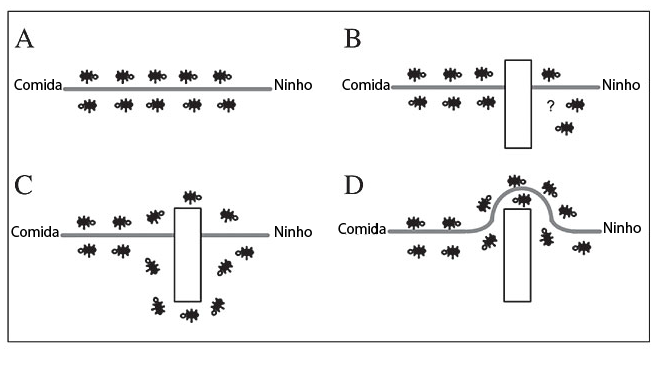
\includegraphics[scale=0.5]{imagens/aco-sample.png}
	\end{center}
	\legend{Fonte: Google Images}
\end{figure}


As formigas conseguem obter um bom caminho entre dois pontos. Na primeira decisão após a inserção do obstáculo, as quantidades de formigas a escolher a rota mais curta e a mais longa devem ser aproximadamente a mesma, de modo que elas fazem suas escolhas com base no feromônio encontrado, sendo que as probabilidades de ambos os lados devem ter valores próximos um do outro. Porém, na segunda decisão, as formigas que percorreram o trajeto mais curto já estão voltando, depositando ainda mais feromônio, enquanto as que foram pelo perscurso mais longo ainda estão completando a primeira transição. Desta forma, as formigas tendem a seguir o mais curto.

De forma análoga, um indivíduo da colônia artificial constrói soluções candidatas, começando com uma solução vazia e, em seguida, adicionando componentes solução de forma iterativa até uma solução candidata completa ser gerada. Após a construção da solução estar completa, as formigas dão feedback das soluções que elas construíram depositando feromônio nos componentes da solução que elas usaram em sua solução. Tipicamente, os componentes da solução que fazem parte de melhores soluções ou são usados por muitas formigas receberão uma maior quantidade de feromônio. Portanto, provavelmente estes componentes serão usados pelas formigas em iterações futuras do algoritmo. Para evitar que a busca fique estagnada, geralmente antes das trilhas de feromônio serem reforçadas, todas as trilhas de feromônio são diminuídas por um fator $\rho$.

Em geral, todos os algoritmos ACO para combinação combinatória estática seguem um esquema algorítmico específico mostrado no Pseudocódigo \ref{alg:aco}. Após a inicialização das trilhas de feromônio e alguns parâmetros, um loop principal é repetido até uma condição de término - que pode ser um certo número de construções de soluções ou um determinado limite de tempo de CPU - é cumprido. No loop essencial, primeiro, as formigas constroem soluções viáveis, então as soluções geradas podem ser melhoradas pela aplicação busca local e, finalmente, as trilhas de feromônios são atualizados.

\begin{algorithm}[H]
	\caption{Ant Colony Optimisation}\label{alg:aco}
	\begin{algorithmic}[1]
		\small
        \State{Configurar parametros, inicializar as trilhas de feromônio}
        \
		\State{Enquanto o critério de parada não é satisfeito:}
        \State{Para cada uma das formgias(em parelelo):}
        \State{Construi soluções}
        \State{Aplique Busca Local (opcional)}
        \State{Atualize as trilhas}
	\end{algorithmic}
\end{algorithm}

Na ACO, as soluções são geradas num processo iterativo no qual agentes inteligentes, as formigas, percorrem todas as
cidades de uma instância de TSP, por exemplo, escolhendo a cada iteração a próxima cidade de sua rota de maneira
estocástica através da Regra de Transição de Estado (RTE). A RTE \cite{dorigo1996any} do Ant Colony Optization é mostrada na Equação \ref{eq:aco-ret}:

\begin{equation} \label{eq:aco-ret} 
    p_i^k = \Bigg\{
        \begin{tabular}{ll}
        \(\frac{[\tau_{ij}(t)]^\alpha[\eta_{ij}]^\beta}{\sum{}^{}{[\tau_{ij}(t)]^\alpha[\eta_{ij}]^\beta}}\), & se $j$ é uma aresta permitida à $k$ \\
        0, & caso contrário
        \end{tabular}
\end{equation}

Na Equação \ref{eq:aco-ret}, que determina a probabilidade de um vértice ser escolhido por uma formiga, $i$ representa o vértice no qual a formiga $k$ se encontra, e $j$ um dos possíveis vértices para o qual ela pode se deslocar. Os vértices permitidos à formiga são aqueles ainda não visitados até a fase atual da construção da solução. Cada formiga armazena os nós já visitados em sua memória, que é denominada como lista tabu. $\tau_{ij}(t)$ corresponde à quantidade de feromônio presente na aresta entre os vértices $i$ e $j$ no instante $t$. $\eta_{ij}$ corresponde à visibilidade da aresta, que é definida pelo valor $1/c_{ij}$ , onde $c_{ij}$ é o custo de deslocamento da aresta. $\alpha$ e $\beta$ são parâmetros que definem o peso da trilha de feromônio e da visibilidade, respectivamente, na escolha do próximo vértice pela formiga \cite{dorigo1996any}.

% ---
\section{ACS}
\label{sec-acs}
% ---

O algoritmo \textit{Ant Colony System}, ou Sistema de Colônia de Formigas, é  uma abordagem derivada da Otimização de Colônia de Formigas (ACO) também desenvolvida por Dorigo et al. (2006) \cite{dorigo2008particle}. O ACS difere do ACO em três pontoss: utiliza uma RTE mais agressiva; a RAF (Regra de Atualização de feromônio) determina que a evaporação e o depósito de feromônio, ao final de cada ciclo, acontecem apenas nas arestas pertencentes à \textit{best-so-far solution}, ou seja, a melhor solução encontrada até o momento em uma execução do algoritmo; e, a cada vez que uma formiga utiliza uma aresta numa solução, uma quantidade pré-definida de feromônio é removida da aresta, para aumentar a exploração de caminhos alternativos. Outra diferençaa importante é em relação ao número $N$ de formigas que percorrem o grafo e constroem suas próprias soluções simultaneamente: enquanto no ACO o melhor valor encontrado experimentalmente é $N = n$, para o ACS o melhor valor encontrado é $N = 10$ \cite{dorigo2008particle}.

\begin{equation} \label{eq:acs-ret} 
    j = \Bigg\{
        \begin{tabular}{ll}
        argmax\(_{l \in J_k} \{\tau_{il}[\eta_{il}]^\beta\}\), & if $q \leq q_0$ \\
        J, & caso contrário
        \end{tabular}
\end{equation}

A RTE do ACS está mostrada na equação 10, na qual $j$ representa a cidade escolhida por uma formiga $k$ que se encontra
no vértice $i$ ao se movimentar. Esta equação é chamada de regra proporcional pseudo-aleatória, pois o parâmetro $q_0$ define a porcentagem das escolhas que serão feitas de forma determinística pelas formigas, onde $0 \leq q0 \leq 1$. Sendo q uma variável aleatória uniformemente distribuída em $[0, 1]$ e atualizada a cada movimento, se $q_0 = 1$, todas as escolhas das formigas serão realizadas de forma determinística, pelo valor máximo de $\tau_{il}[\eta_{il}]^\beta$, onde $l \in S_k^i$ corresponde ao conjunto de cidades permitidas à formiga no movimento. Se, ao contrário, $q_0 = 0$, todas as escolhas serão realizadas de forma estocástica, pois $J$ representa uma cidade escolhida através das probabilidades calculadas pela Equação \ref{eq:aco-ret}, com a única diferença que o parâmetro $\alpha$ foi excluído, ou seja, seu valor foi fixado em 1. O melhor valor definido experimentalmente é $q_0 = 0.9$, o que significa que 90\% das escolhas serão determinísticas \cite{dorigo2008particle}.

De acordo com Dorigo et al \cite{dorigo2008particle}, a RAF do ACS define que a atualização de feromônio ocorre em dois momentos: uma atualização global, ao final de cada ciclo do algoritmo; e uma atualização local, logo depois que uma formiga se move de uma cidade a outra, ou seja, inclui mais uma aresta na sua rota. A regra para Atualização Global de Feromônio (AGF) está apresentada nas Equações \ref{eq:acs-agf1} e \ref{eq:acs-agf2}, onde $\rho$ é o coeficiente de persistência do feromônio, cujo melhor valor encontrado para o ACS é $\rho = 0.1$. $T^{bs}$ corresponde ao conjunto de arestas que fazem parte da melhor solução encontrada até o momento atual da execução do algoritmo e $C^{bs}$ corresponde ao custo de $T^{bs}$.

\begin{equation} \label{eq:acs-agf1} 
    \tau_{ij} = (1 - \rho)\tau_{ij} + \rho\Delta\tau_{ij}^{bs}, \forall (i,j) \in T^{bs}, 
\end{equation}

\begin{equation} \label{eq:acs-agf2} 
    \Delta\tau_{ij}^{bs} = 1/C^{bs}
\end{equation}

A regra de Atualização Local de Feromônio (ALF) \cite{dorigo2008particle} está apresentada na Equação \ref{eq:acs-alf}, na qual $\xi$ é um parâmetro cujo melhor valor experimentalmente calculado é $\xi = \rho = 0.1$. $\tau_0$ também é um parâmetro que, além de ser utilizado na atualização local de feromônio, também corresponde à quantidade de feromônio depositada em todas as arestas no início da execução do algoritmo. O melhor valor encontrado para $\tau_0$ é calculado a partir do custo de uma solução criada aplicando um algoritmo do vizinho mais próximo à instância em análise. A fórmula para cálculo de $\tau_0$ é mostrada na Equação \ref{eq:acs-tau}, na qual $n$ é igual ao número de cidades da instância e $C^{nn}$ é igual ao custo da solução obtido utilizando um algoritmo do vizinho mais próximo sobre a instância.

\begin{equation} \label{eq:acs-alf} 
    \tau_{ij} = (1 - \xi)\tau_{ij} + \xi\tau_0,
\end{equation}

\begin{equation} \label{eq:acs-tau} 
    \tau_0 = 1/nC^{nn}
\end{equation}

% ---
\section{TACO}
\label{sec-taco}
% ---

A Otimização de Colônia de Formigas por Times (TACO), proposta por Vallivaara (2008) \cite{vallivaara2008team}, é baseada no ACS (\textit{Ant Colony System}) para resolver instâncias de MTSP (\textit{Multiple Travelling Salesmen Problem}). Essa generalização básica é feita substituindo as $N$ formigas ACS, que constroem soluções para o TSP, com $N$ equipes de $m$ membros, fazendo um total de formigas igual a $N \times m$. Uma equipe de formigas representa um vendedor na construção da solução MTSP e cada equipe tem sua lista de tabu.

A única diferença entre o ACS e o TACO com $m = 1$ é que no primeiro as formigas podem ser colocadas nos nós aleatoriamente no estágio inicial. Como isso não é possível no TACO e no MTSP, é natural que as formigas sejam colocadas inicialmente nos pontos de partida iniciais \cite{vallivaara2008team}. Para distribuir a carga de trabalho, uma formiga com a rota parcial mais curta escolhe sua próxima cidade $j$, em qualquer momento do processo de construção, de acordo com a equação da Regra de Estado de Transição (RET), conforme mostrado em \ref{eq:taco-ret}.

\begin{equation} \label{eq:taco-ret} 
    j = \Bigg\{
        \begin{tabular}{ll}
        argmax\(_{l \in J_k} \{\tau_{il}[\eta_{il}]^\beta\}\), & if $q \leq q_0$ \\
        J, & caso contrário
        \end{tabular}
\end{equation}

Durante a fase de inicialização, o nível de feromônio é ajustado para $\tau_0 = 1 / nC^{nn}$ em cada aresta, como sugerido no ACS. Antes de começar a construção da rota, todos os nós são configurados como não-visitados por cada equipe. Em seguida, cada membro $m$ de uma equipe $N_i$ é colocado na cidade inicial correspondente $v_k$, e todas as cidades iniciais são marcadas como visitadas para este mesmo time \cite{vallivaara2008team}.

Estando uma formiga $k$ posicionada em um vértice $v_k$; sendo $v_0$ o depósito da instância; $c(v_i, v_j)$ o
custo de deslocamento entre dois vértices $v_i$ e $v_j$ quaisquer; o Custo Parcial total $CP(k)$ da rota já percorrida pela formiga $k$; e tendo sido escolhido o vértice $v_j$ como seu próximo vértice de acordo com a equação \ref{eq:taco-ret}; o método consiste em verificar, antes da formiga de mover, se existe qualquer outra formiga $l$ da instância que respeite a inequação \ref{eq:taco-custo-parcial}. Se houver, então é permitido que a formiga $l$ escolha seu próximo vértice novamente de acordo com a RET presente em \ref{eq:taco-ret}, e se movimente para o novo vértice escolhido \cite{vallivaara2008team}.

\begin{equation} \label{eq:taco-custo-parcial} 
    c(v_l, v_j) + c(v_j , v_0) + CP(l) < c(v_k, v_j) + c(v_j , v_0) + CP(k)
\end{equation}

TACO tem vários parâmetros que são responsáveis pelo seu comportamento durante a construção de soluções. A probabilidade inicial $q_0$ determina se a inicialização das formigas tem apenas escolhas determinísticas ou aleatórias $(0 < q_0 <1)$. Os parâmetros de feromônio $\alpha$ e $\beta$ definem o peso da trilha de feromônio e a visibilidade, respectivamente, na escolha do próximo nó pela formiga. O parâmetro $\xi$ controla a persistência do feromônio quando a Regra de Atualização de Feromônio (RAF) ocorre localmente, logo após uma formiga se mover de uma cidade para outra, ou seja, inclui mais uma borda em sua rota. Da mesma forma, $\rho$ regula a persistência de feromônios para RAF global, ou seja, no final de cada ciclo do algoritmo.

Finalmente, o algoritmo usa uma abordagem de pesquisa local para melhorar as soluções construídas. A pesquisa local opt-2 altera quaisquer duas arestas de uma solução e verifica se ela obtém alguma melhoria. O procedimento opt-2 é aplicado a todas as soluções construídas \cite{vallivaara2008team}.

% ---
\section{PSO}
\label{sec-pso}
% ---

Kennedy e Eberhart (1999) \cite{kennedy1999particle} propuseram o método \textit{Partition Swarm Optimization} (PSO) baseado no revoada das aves. O PSO é adequado para a otimização de variáveis contínuas em um espaço de busca de alta dimensão e apresenta alta precisão. Ele realiza a pesquisa por meio de um enxame de partículas por meio de um processo de iteração.

Cada partícula se move em direção a sua melhor posição ($P_{best}$) anterior e a melhor posição global ($G_{best}$) no enxame para alcançar a solução ótima, como mostrado na Equação \ref{eq:pso-movement}.

\begin{equation} \label{eq:pso-movement}
    \vec{x}_{i(t+1)} = \vec{x}_{i(t)} + \vec{v}_{i(t)}
\end{equation}

A solução representa a posição da partícula no espaço de busca, um vetor $\vec{x}_i$. Para cada etapa, as partículas têm suas posições de acordo com seu vetor de velocidade $\vec{v}_i$, como mostrado na Equação \ref{eq:pso-speed}, encontrado no trabalho de Shi \cite{shi1998modified}.

\begin{equation} \label{eq:pso-speed}
    \vec{v}_j = \omega \vec{v}_j + c_1 r_1(P_{best} - \vec{x}_j) + c_2 r_2(G_{best} - \vec{x}_j)
\end{equation} 

onde $c_1$ e $c_2$ são números positivos constantes (sendo $c_1$ é referente ao comportamento cognitivo e $c_2$ ao comportamento social); $r_1$ e $r_2$ são números aleatórios entre o intervalo $[0,1]$.

A velocidade de fixação, um limite superior para o parâmetro de velocidade evita que as partículas voem para fora do espaço de busca. Da mesma forma, a estratégia do "coeficiente de constrição", proposta por Clerc e Kennedy (2008) \cite{clerc2002particle}, constrói as velocidades através da análise dinâmica de enxames.

A inércia, mostrada na primeira parte da Equação \ref{eq:pso-clerc-speed}, representa a velocidade anterior, que fornece o momento necessário para as partículas percorrerem o espaço de busca.

\begin{equation} \label{eq:pso-clerc-speed}
    \vec{v}_{ij}(t+1) = \chi[\vec{v}_{ij}(t+1) + \varphi_1(\vec{v}_{ij}(t) - \vec{x}_{ij}(t)) + \varphi_2(\hat{y}_{ij}(t) - \vec{x}_{ij}(t))]
\end{equation}

Por outro lado, o componente cognitivo, a Equação \ref{eq:pso-clerc}, determina o movimento individual de cada partícula. Ele incentiva as partículas a se moverem em direção às suas melhores posições atuais. 

\begin{equation} \label{eq:pso-clerc}
    \chi = \frac{2}{4 - \varphi - \sqrt{\varphi^2 - 4\varphi}}
\end{equation}

A último a Equação \ref{eq:pso-clerc-coefficient}, o componente "social", implica o efeito colaborativo das partículas para encontrar a solução global ótima.

\begin{equation} \label{eq:pso-clerc-coefficient}
    \varphi = \varphi_1 + \varphi_2
\end{equation}

onde $ \varphi_1 = c_1$ e $ \varphi_2 = c_2$.

% \begin{algorithm}
% 	\caption{Particle Swarm Optimization}\label{alg:pso}
% 	\begin{algorithmic}[1]
% 		\small
% 		\State{Inicializar a posição \(x_i\), a velocidade \(v_i\) e a melhor posição pessoal \(P_{best}\) das \(N\) partículas}
%         \State{Enquanto o critério de parada não é satisfeito faça}
%         \State{Para \(j = 1\) até \(N\) faça:}
%         \State{\(G_{best}\) = }
%         \State{Análise dos resultados via gráficos e mapas de calor}
% 	\end{algorithmic}
% \end{algorithm}

% ---
\section{FSS}
\label{sec-fss}
% ---

Bastos-Filho et al. (2008) \cite{bastos2008novel} desenvolveu um algoritmo de busca de base populacional inspirado no comportamento de natação de peixes, que se expande e se contrai enquanto procura comida. O algoritmo \textit{Fish School Search} (FSS) considera os movimentos individuais e coletivos dos peixes. Esse algoritmo de otimização não apresenta a mesma capacidade de exploração do PSO, mas tem a capacidade de encontrar boas soluções em um espaço de pesquisa com muitos mínimos locais.

Cada peixe, em localização $n$-dimensional, representa uma solução viável para o problema. Seu sucesso é medido pelo seu peso, uma conta cumulativa do sucesso da busca por cada peixe na escola. Os peixes não apenas armazenam informações sobre seu peso, mas também se posicionam no espaço de busca.

O FSS consiste em operadores de movimentação e alimentação. No movimento individual, cada peixe se desloca aleatoriamente em direção a uma posição em sua vizinhança à procura de regiões promissoras. Este componente é calculado usando a Equação \ref{eq:fss-movement}.

\begin{equation} \label{eq:fss-movement}
    \vec{n}_{i}(t) = \vec{x}_{i(t-1)} + step_{ind} \times rand[-1,1]
\end{equation}

onde $\vec{n}_{i}(t) $ representa o novo vetor posição do peixe na dimensão $i$, $ \vec{x}_{i(t)} $  a posição atual, $ step_{ind} $ sendo o passo individual e $ rand[-1,1]$ um número aleatório gerado por uma distribuição uniforme no intervalo $[-1; 1]$.

Após o movimento individual é necessário calcular a diferença entre o \textit{fitness} dos indivíduos, de acordo com \ref{eq:fss-fit}:

\begin{equation} \label{eq:fss-fit}
    \Delta f_{i}(t) = f[\vec{n}_{i}(t)] - f[\vec{x}_{i}(t-1)]
\end{equation}

onde $f[\vec{x}_{i}(t)]$ é o \textit{fitness} do indivíduo atual e $f[\vec{n}_{i}(t)]$ é o fitness do próximo indivíduo.

Depois de se mudar para novas posições, todos os peixes têm seus pesos atualizados de acordo com a Equação \ref{eq:fss-feeding}. A atualização de peso é determinada pelo sucesso do movimento individual, que é calculado através da adequação das posições atual e nova.

\begin{equation} \label{eq:fss-feeding}
    W_{i(t)} = W_{i(t-1)} + \frac{\Delta f_{i(t)}}{max[\Delta f_{i(t)}]}
\end{equation}

onde $W_{i}(t)$ é o peso atual do indivíduo.

Depois de alimentar todos os peixes, ocorre o movimento coletivo-instintivo. Todos os peixes se movem em direção a um vetor de influência, como mostrado nas Equações \ref{eq:fss-fitness} e \ref{eq:fss-newmove}. Os peixes que melhoraram sua aptidão na iteração atual e geram esse vetor.

\begin{equation} \label{eq:fss-fitness}
    \vec{m}_{i(t)} = \frac{\sum_{}^{} N_i = \vec{x}_{i(t)} \times W_{i(t)}}{\sum_{}^{} N_i = W_{i(t)}}
\end{equation}

onde $\Delta x_{i}(t)$ é o deslocamento do peixe gerado pelo movimento individual.

\begin{equation} \label{eq:fss-newmove}
    \vec{x}_{i(t)} = \vec{x}_{i(t-1)} + \vec{m}_{i(t)}
\end{equation}

No final da iteração atual, o cardume se contrai ou se expande de acordo com o operador do movimento volitivo-coletivo. A contração da escola resulta em uma busca de exploração, enquanto sua expansão faz com que a escola explore a área de busca, evitando os mínimos locais. Assim, o operador volitivo calcula o baricentro da escola como mostrado na Equação \ref{eq:fss-barycentre} e atualiza o seu movimento, de acordo com a Equação \ref{eq:moveagain}. Este último operador fornece ao FSS a capacidade de auto-ajustar a granularidade da pesquisa ao longo do processo de otimização.

\begin{equation} \label{eq:fss-barycentre}
    \vec{B}_i = \frac{\sum_{}^{} \vec{x}_{i}(t)W_{i}(t)}{\sum_{}^{} W_{i}(t)}
\end{equation}

\begin{equation} \label{eq:moveagain}
    \vec{x}_{i}(t) = \vec{x}_{i}(t) \pm step_{vol}\frac{\vec{x}_{i}(t) - \vec{B}_i}{dist(\vec{x}_{i}(t), \vec{B}_i)}
\end{equation}

onde $dist[]$ é uma função que retorna a distância euclidiana entre a posição do peixe e o baricentro, e $step_{vol}$ é um passo para controlar o deslocamento do movimento.


% ---
\section{MOFSS}
\label{sec-mofss}
% ---

A \textit{Multi-Objective Fish School Search} (MOFSS) é uma generalização FSS que lida com problemas com múltiplas restrições objetivas. Ele usa um Arquivo Externo (EA) para armazenar as melhores soluções não dominadas encontradas durante o processo de busca. As soluções no EA são usadas para guiar os movimentos dos peixes no espaço de busca. O método \textit{Crowding Distance} trunca o EA para lidar com seu limite de tamanho. O MOFSS difere do FSS nos operadores de seleção de recursos que são adaptados para resolver problemas multi-objetivos.

No movimento individual, o peixe sempre se move em direção a novas posições, mesmo que sejam piores que as anteriores ou as posições sejam indiferentes, considerando o critério de dominância. Soluções no EA levam os movimentos individuais. Para cada peixe, um guia é selecionado usando o operador de seleção de líder. A seleção é executada por um torneio que seleciona dois peixes e executa uma seleção aleatória para retornar um guia.

A nova posição do pexei é calculada através da Equação \ref{eq:mofss-movimento}:

\begin{equation} \label{eq:mofss-movimento}
    \vec{n}_{i}(t) = \vec{x}_{i}(t) + \Delta\vec{x}_{i}(t)
\end{equation}

Em que $\vec{x}_{i}(t)$ é a posição atual do peixe $i$, $\vec{n}_{i}(t) $ é a nova posição e $\Delta\vec{x}_{i}(t)$ é o deslocamento, calculado através da Equação \ref{eq:mofss-deslocamento}:

\begin{equation} \label{eq:mofss-deslocamento}
    \Delta\vec{x}_{i}(t) = S_{ind}(t) \times U[0,1] \times \frac{\vec{x}_{g}(t) - \vec{x}_{i}(t)}{DIST[\vec{x}_{g}(t), \vec{x}_{i}(t)]}
\end{equation}

Onde $S_{ind}(t)$ é o passo individual, $U[0,1]$ é uma distribuição uniforme aleatória entre 0 e 1 e $DIST[\vec{x}_{g}(t), \vec{x}_{i}(t)]$ é uma função que calcula a distância euclidiana.

O operador de alimentação é quem define o conhecimento do cardume, atualizando o peso de cada peixe conforme seu movimento individual e, consequentemente, atualizando o peso total do cardume. Diferentemente da versão mono-objetiva do FSS (\textit{Fish School Search}), nesta abordagem há varios objetivos conflitantes entre si e por isso é preciso utilizar um conceito de dominância para determinar qual e a melhor solução \cite{bastos2015multi}. Para tanto, é necessário possuir dois elementos, a posição atual do peixe $x_{i}(t)$ e a nova posição do peixe $n_{i}(t)$, determinada pelo operador de de movimento individual \cite{bastos2015multi}.

Para determinar se o peixe ira sofrer um aumento ou um diminuição de peso, foi introduzido a verificação do valor de \textit{Crowding Distance} da solução do arquivo externo que está mais proxima da posição atual do peixe e da solução do arquivo externo que esta mais proxima da nova posição deste \cite{bastos2015multi}.

Um fator de grau de domínio $D_{i}(t)$ também foi introduzido ao cálculo do peso do peixe. Este grau de domínio é determinado através da análise da quantidade de soluções que um peixe domina e da quantidade de soluções que dominam este mesmo peixe. Com isso, cria-se uma variável que prioriza o aumento do peso dos peixes que estão mais próximos do arquivo externo e penaliza os que se encontram mais distantes \cite{bastos2015multi}.

O fator de dominânia $D_{i}(t)$ é cálculo de acordo com a Equação \ref{eq:mofss-dominio}:

\begin{equation} \label{eq:mofss-dominio}
    D_{i}(t) = 1 - \frac{R_{i}}{MaxR}
\end{equation}

em que $R(i)$ representa a aptidão (ou \textit{fitness}) bruta do peixe e $MaxR$ é o máximo valor de aptidão bruta encontrado na iteração. A aptidão bruta $R(i)$ é calculado através da equação Equação \ref{eq:mofss-aptidao-bruta}, 

\begin{equation} \label{eq:mofss-aptidao-bruta}
    R_{i} = \sum_{j \in N, j \prec i} S(j)
\end{equation}

onde $S(j)$ é um valor de forçaa e representa o número de soluções que peixe $j$ domina, calculado conforme a Equação \ref{eq:mofss-forca}:

\begin{equation} \label{eq:mofss-forca}
    S(i) = |{j | j \in N \wedge i \prec j}|
\end{equation}

Depois do cálculo do grau de domínio, cada peixe tem seu valor de peso atualizado conforme a Equação \ref{eq:mofss-alimentacao}:

\begin{equation} \label{eq:mofss-alimentacao}
    w_{i}(t + 1) = w_{i} + \Delta w_{i}(t) \times D_{i}(t)
\end{equation}

E o peso total do cardume na iteração atual é calculado através da Equação \ref{eq:mofss-pesocardume}:

\begin{equation} \label{eq:mofss-pesocardume}
    w(t + 1) = \sum_{i=1}^{N} w_{i}(t+1)
\end{equation}

O movimento volitivo multi-objetivo leva o conjunto de soluções não dominadas da EA (Arquivo Externo) como pontos de referência para contratar ou expandir o cardume, enquanto o FSS usa o baricentro escolar para determinar esses pontos. Cada peixe da escola seleciona um líder, usando o operador de seleção de líderes, e se move em direção a ele. Assim, os peixes tendem a se mover para as soluções não dominadas \cite{bastos2015multi}.

O operador de movimento coletivo instintivo é responsável por fazer o cardume sofrer um deslocamento, influenciado pelo desempenho geral obtido por cada peixe em seu operador de movimento individual. Dois modos distintos são utilizados para determinar o vetor de influência coletiva instintiva. No primeiro modo, este vetor é calculado (ver Equação \ref{eq:mofss-institivo-i}) igualmente para todo o cardume, ou seja, todos os peixes possuem o mesmo valor de infuência:

\begin{equation} \label{eq:mofss-institivo-i}
    \vec{I}(t) = \sum_{i=1}^{N} \frac{\Delta w_{i}(t) \times \Delta \vec{x}_{i}(t)}{MAX[1, (\Delta w)]}
\end{equation}

Já na segunda opção, cada peixe tem um vetor de influência determinado individualmente (ver Equação \ref{eq:mofss-institivo-ii}), como base no seu ganho de peso na iteração atual:

\begin{equation} \label{eq:mofss-institivo-ii}
    \vec{I}(t) = S_{vol}(t) \times U[0,1] \times \Delta w_{i}(t) \frac{\vec{x}_{i}(t) - \vec{x}_{g}(t)}{DIST[\vec{x}_{i}(t), \vec{x}_{g}(t)]}
\end{equation}

Sendo as posições dos peixes atualizados através da Equação \ref{eq:mofss-institivo-iii} em ambas abordagens.

\begin{equation} \label{eq:mofss-institivo-iii}
    \vec{x}_{i}(t + 1) = \vec{x}_{i}(t) + \vec{I}(t)
\end{equation}

Por fim, o operador de movimento coletivo volitivo determina se o cardume deve se movimentar para realizar uma busca em amplitude ou uma busca em profundidade. Para tanto é calculado um vetor de influência volitiva (ver Equação \ref{eq:mofss-volitivo-i}), que é adicionado a cada peixe do cardume, fazendo que eles se desloquem para uma nova posição \cite{bastos2015multi}.

\begin{equation} \label{eq:mofss-volitivo-i}
    V_{i}(t) = S_{vol}(t) \times SINAL(\Delta w) \times U[0,1]
\end{equation}

onde $SINAL(\Delta w)$ é uma função que determina o sinal dos valores informados, retornando 1 caso o valor seja positivo ou -1 caso o valor seja negativo.

Como consequência, as posições dos peixes atualizados através da Equação \ref{eq:mofss-volitivo-ii}.

\begin{equation} \label{eq:mofss-volitivo-ii}
    \vec{x}_{i}(t + 1) = \vec{x}_{i}(t) + V_{i}(t) \times \frac{\vec{x}_{i}(t) - \vec{x}_{g}(t)}{DIST[\vec{x}_{i}(t), \vec{x}_{g}(t)]}
\end{equation}

Finalmente, o operador de turbulência ocorre para evitar que o enxame fique preso nos mínimos locais. O operador cria novas posições vizinhas que são avaliadas em cada iteração. Se as novas posições forem soluções não dominadas, elas serão incluídas no EA.
